% Created 2012-10-08 Mon 20:56
\documentclass[11pt]{article}
\usepackage[latin1]{inputenc}
\usepackage{fixltx2e}
\usepackage{url}
\usepackage{graphicx}
\usepackage{minted}
\usepackage{color}
\usepackage{longtable}
\usepackage{float}
\usepackage{wrapfig}
\usepackage{soul}
\usepackage{textcomp}
\usepackage{amsmath}
\usepackage{marvosym}
\usepackage{wasysym}
\usepackage{latexsym}
\usepackage{amssymb}
\usepackage[linktocpage,
  pdfstartview=FitH,
  colorlinks,
  linkcolor=blue,
  anchorcolor=blue,
  citecolor=blue,
  filecolor=blue,
  menucolor=blue,
  urlcolor=blue]{hyperref}
\usepackage{attachfile}
\tolerance=1000
\usepackage{adjustbox}
\usepackage{anysize}
\marginsize{1in}{1in}{1in}{1in}
\providecommand{\alert}[1]{\textbf{#1}}

\title{Literature Review: Using DFT to study active surfaces in the oxygen evolution reaction (OER)}
\author{Zhongnan Xu}
\date{10/08/12 Monday}
\hypersetup{
  pdfkeywords={},
  pdfsubject={},
  pdfcreator={Emacs Org-mode version 7.8.11}}

\begin{document}

\maketitle



\section{Introduction}
\label{sec-1}

  The specific problem addressed is how to accurately represent active
  surfaces of oxides in the oxygen evolution reaction (OER).
  This problem is relevant because of a recently developed atomistic 
  thermodynamic framework for studying OER.
  This framework allows us to calculate theoretical activities of oxides in 
  OER off of the adsorption energies of *O, *OH, and *OOH. 
  Initial studies of these mechanisms were done on ideal surfaces with
  an arbitrary coverage of intermediates, and water was not assumed to
  naturally dissociate onto these surfaces.
  
  Recently, two papers from separate research groups have attempted to
  build on this theory to more accurately mimic actual oxide surfaces
  in water.
  The two papers are titled ``Identifying active surface phases for metal oxide
  electrocatalysts: a study of manganese oxide bi-functional catalysts
  for oxygen reduction and water oxidation catalysis'' and ``Water
  Oxidation on Pure and Doped Hematite (0001) Surfaces: Prediction of Co
  and Ni as Effective Dopants for Electrocatalysis'', and their
  corresponding authors are Jan Rossmeisl and Emily A. Carter,
  respectively.
  Detailed references can be seen in the footnotes and the full article
  can be found in the folder with this assignment.\footnote{Su, H.; Gorlin, Y.; Man, I. C.; Calle-vallejo, F.; Norskov, J. K.;
Jaramillo, F.; Rossmeisl, J. Physical Chemistry Chemical Physics 2012,
14, 14010
 }\textsuperscript{,}\,\footnote{Liao, P.; Keith, J. A; Carter, E. A Journal of the American Chemical
Society 2012, 134, 13296
 }
  
\section{Methods}
\label{sec-2}

  Both article's overall goal was to evaluate catalyst's performance in
  the oxygen evolution reaction (OER) using the same atomistic framework
  constructed in a previous article \footnote{Man, I.; Su, H.; Calle-Vallejo, F. ChemCatChem 2011, 3, 1159
 }.
  Both articles took the basic framework established and used it to
  look at two different systems (MnO$_{x}$ and Fe$_{2}$O$_{3}$) with two
  different goals.
  Rossmeisl's goal was to model both the thermodynamics and
  kinetics of OER and construct a theoretical current-voltage curve,
  while Carter's goal was to compare only the thermodynamics of pure and
  doped hematite for photovoltaic applications.
  In accomplishing goals, both articles opted to include the effects
  of water dissociation on an idealized surface, and I will only focus
  on this aspect of both articles for the literature review. 
\subsection{Rossmeisl Approach: Effects of pH and electrode potential}
\label{sec-2-1}

   Rossmeisl's goal was to construct a current-voltage curve of the
   performance of the MnO$_{x}$ system in both oxygen evolution and
   reduction and compare this to experiments to help elucidate
   possible mechanims and surfaces.
   Therefore, they had to add in effects of pH and varying electrode
   potential.
   They did this by taking a bulk Pourbaix diagram and `upgrading' it 
   to include surface coverages with respect to pH and applied potential.
   They studied the MnO$_{x}$ system in OER conditions, which included
   Mn$_{3}$O$_{4}$, Mn$_{2}$O$_{3}$, and MnO$_{2}$.
   Their goal was to use DFT to find both thermodynamic and kinetic data
   and model a fully self-consistent current-voltage curve of a MnO$_{x}$
   electrode and compare them qualitatively to experiments.
   In order for this curve to be self-consistent, they had to take into
   account changes of both bulk \textbf{and} surface phases with respect to
   applied potential and pH.
   Their main equation of modeling dissociation and adsorption of water
   onto each of the idealized surfaces is shown below.
   
   \begin{equation}
   \begin{split}
   X^\ast &+ (N_{\mathrm{O^\ast}} + N_{\mathrm{HO^\ast}})\mathrm{H_2O}(l)
   \rightarrow \\
   & (N_{\mathrm{O^\ast}} + N_{\mathrm{HO^\ast}} +
   N^\ast)_{\mathrm{ads}} + (2N_{\mathrm{O^\ast}} +
   N_{\mathrm{HO^\ast}})\mathrm{H^+} + (2N_{\mathrm{O^\ast}} + N_{\mathrm{HO^\ast}})\mathrm{e^-}
   \end{split}
   \end{equation}
   
   This reaction describes the interaction of water with
   surfaces. 
   Starting with a clean surface with a total of $X^\ast$ sites, water 
   will adsorb and produce protons, electrons, and adsorbed
   species of either $\mathrm{O^{\ast}}$ or $\mathrm{HO^{\ast}}$. 
   In producing these intermediates, there will be a release of an 
   electron and proton, and higher pHs and higher applied potentials 
   will preferentially stabilize coverages with more of these
   intermediates.
   The Gibbs free energy of a surface under these conditions is shown
   below.
   
   \begin{equation}
   \begin{split}
   G_{\mathrm{surf}} &= E_{(N_{\mathrm{O^\ast}} + N_{\mathrm{HO^\ast}} + N_\ast)_{\mathrm{ads}}} - E_{\mathrm{X^{\ast}}} -
   (N_{\mathrm{O^\ast}} + N_{\mathrm{HO^\ast}}) E_{\mathrm{H_2O(g)}} \\ 
   &\quad + \dfrac{2N_{\mathrm{O^\ast}} +
   N_{\mathrm{HO^\ast}}}{2} E_{\mathrm{H_2(g)}} + \mathrm{\Delta ZPE -
   T\Delta S} \\
   &\quad - (2N_{\mathrm{O^\ast}} + N_{\mathrm{HO^\ast}})(eU +
   k_\mathrm{B}T\mathrm{ln}10\mathrm{pH})
   \end{split}
   \end{equation}
   
   To use this equation, one models the same surface with different
   coverages of O and OH. Generally, the more adsorbates on the surface,
   the more free electrons and protons that need to be produced, and the
   more likely that surface will be present at higher potentials and
   pH's.

   To implement this in predicting active surface phaes, they would
   first graph the relationship between applied voltage and Gibbs free
   surface energy of the surfaces they were investigating. 
   For each of their close packed surfaces, they computed total
   energies with numerous different adsorbates on, including mixtures 
   of OH and O groups.
   Figure 1 shows a sample.

   \begin{figure}[H]
   \centering
   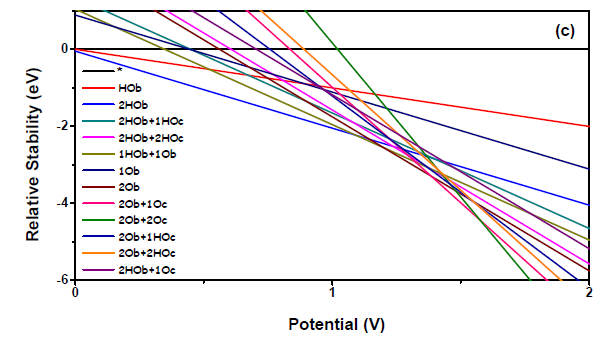
\includegraphics[width=0.7\textwidth]{./rossmeisl-sample.png}
   \caption{\label{fig:constant-pH-free-energy}The phase diagram of MnO$_{2}$(110) surface calculated as function of the potential at pH=0. The notations b and c indicate bridge sites and coordinated unsaturated sites}
   \end{figure}

   This is done at pH=0, and at higher pHs, surfaces with more OH and
   O adsorbed would become lower because of the proton released in the
   adsorption.
   Graphs like this were also done for Mn$_{3}$O$_{4}$(001) and
   Mn$_{2}$O$_{3}$ (110), which can be found in the supplementary data.

   Note that these surface Pourbaix diagrams are done in the context
   of a specific bulk Pourbaix diagram. 
   From experiments, the bulk Pourbaix diagrams are assumed to be
   true, and then in each bulk region of the Pourbaix diagrams, 
   the surface Pourbaix diagrams are constructed. 
   For example, the above graph does not this show this,
   but at a high enough potential, the manganese oxide will naturally
   be converted into MnO$_{4}$$^{-}$.
   Therefore, above a certain potential, the predictes coverages above
   would be meaningless.
   The above graph can then be `mapped onto' a region on the
   experimentally attained bulk Pourbaix diagram to give more
   information on active surface phases. The example for MnO$_{2}$ is
   shown in figure 2.

   \begin{figure}[H]
   \centering
   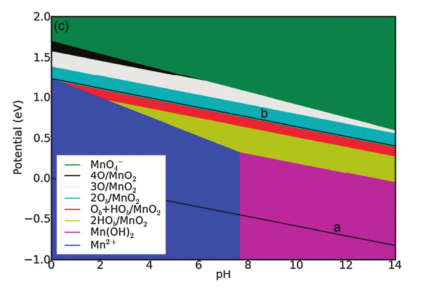
\includegraphics[width=0.7\textwidth]{./pourbaix-mno2.png}
   \caption{\label{fig:MnO_{2}-pourbaix}The bulk and surface Pourbaix diagram of MnO$_{2}$(110) surface}
   \end{figure}
   
   Their final step was combining the Pourbaix diagrams of
   Mn$_{3}$O$_{4}$, Mn$_{2}$O$_{3}$, and MnO$_{2}$ to make a general MnO$_{x}$
   diagram that would predict both the active bulk \textbf{and} surface phase
   at varying potentials and pH. Details of this procedure can be
   found in the attached supplementary information. I chose not to go
   over the details of this procedure out of time and space constraints.
   
\subsection{Carter Approach: A detailed investigation on water dissociation}
\label{sec-2-2}

   Carter et al. (2012) studied hematite (Fe$_{2}$O$_{3}$) for
   photocatalytic water splitting.
   In order to attain a general idea of the surface, they did an
   extensive literature review of both experimental and computational
   investigations on the active surface facet and termination of hematite
   in wet conditions.
   They found that in water, the most likely surface is an
   H$_{3}$-O$_{3}$-Fe-Fe-R surface. 
   
   They opted to not include effects of pH and increasing electrode 
   potential, but did a far more extensive study on possible
   configurations of possible surface configurations.
   Starting with an ideal, oxygen terminated surface of hematite, 
   they asked the question, ``If we were to make surface with dangling 
   hydroxyl groups, which would be most stable? How many of these
   oxygens would be hydrated to make hydroxyl's, and what would the
   configuration of these groups be?'' 
   To answer this question, they first broke up their surface into a 7x7
   grid of a total of 49 points. 
   They then placed one hydrogen atom at each of these points at a height
   of 0.8 $\AA$ above the surface, allowed the hydrogen to
   relax.
   They would then calculate the adsorption energy as shown below.
   
   \begin{equation}
   \begin{split}
   G_{\mathrm{ads}} &= [E(\mathrm{O-terminated\;slab} + n\mathrm{H}) \\
   &\quad E(\mathrm{O-terminated\;slab}) - (n/2)E_{\mathrm{H_2}}]/n \\
   &\quad + \mathrm{\Delta ZPE} - T\Delta S
   \end{split}
   \end{equation}
   
   They then took the structure with the lowest energy and then did the
   same process again with a second hydrogen atom. 
   By doing this, they could be confident that they are getting the
   DFT predicted ground state of their system, and they could also
   systematically analyze increasing coverages of hydroxyl groups.
   Note that equation (3) is independent of how many hydroxyl groups are
   on, so it is possible to find the ground state structure over
   different coverages of hydroxyl groups.
   Figure 3 shows the ground state surfaces at multiple covergaes of
   HO groups.

   \begin{figure}[H],
   \centering
   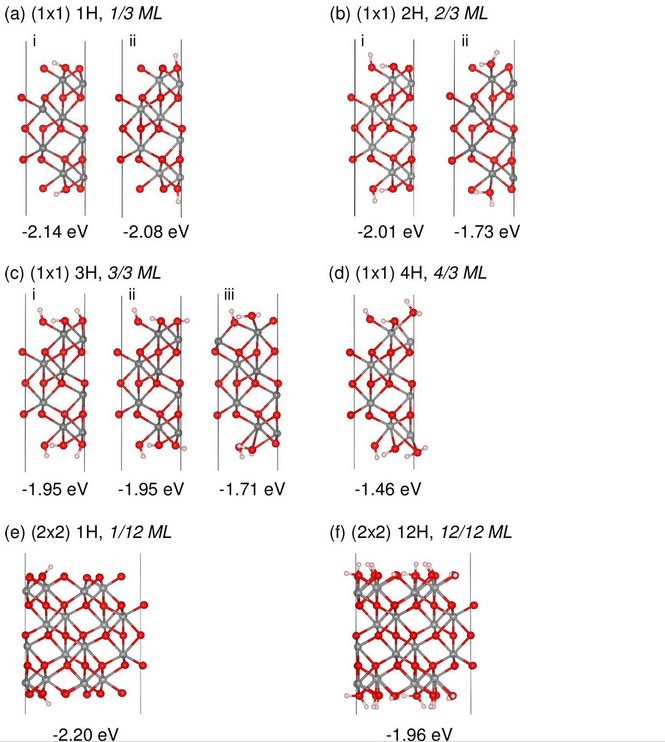
\includegraphics[width=4.5in]{./carter-OH.png}
   \caption{\label{fig:carter-oh}Lowest energy configurations of HO surfaces at multiple coverages and hydrogen adsorption energies.}
   \end{figure}

   In addition to finding the most stable H$_{x}$-O-Fe-Fe-R surface, they
   also included affects of a monolayer of water.
   The orientations of the water molecules were chosen to maximize
   hydrogen bonding, and similar to the procedure for choosing the most
   stable hydroxylated surface, the most stable solvated surface, after
   relaxation, was chosen as well.

   Finally, in calculating adsorption energies of O*, HO* and HOO*,
   they images on which adsorbates would be involved in the reaction.
   This image can be found in the attached article.
   
\section{Discussion}
\label{sec-3}

  When assessing both techniques of accurately representing the
  surface phase in OER conditions, its important note the different
  goals of both.
  Rossmeisl and coworkers were seeking theoretical current-voltage
  curves that could be directly comparable to experiments.
  The purpose of this was to use theoretical techniques to probe the
  fundamental characteristics of active phase
  as one increased the potential in a typical OER experiment.
  Hence, Rossmeisl would need to take into account the relationship
  between bulk/surface stability with potential and pH.
  In contrast, Carter was seeking qualitative agreement between pure
  and doped hematite surfaces.
  Therefore, one could easily assume changes in the bulk and surface
  structures at differing pH's and voltages would not be drastically
  different across different dopings of cations.

  To reproduce these results, the most difficult calculation to
  reproduce geometries of adsorbed intermediates (HO* and HOO*).
  From personal experience, these geometries are 
  highly dependent on their initial, pre-relaxed states.
  Rossmeisl does not describe the geometry of the HO* and HOO*
  adsorbates, furthermore, it is evident from the supplementary data of
  Rossmeisl's paper that he and coworkers performed adsorption energy
  calculations of O*, HO*, and HOO* on at least 50 different
  surfaces, and it is unclear how these adsorption energies were
  calculated in lieu of different coverages. 

  In contrast, Carter's paper gives a clear explanation on how the
  hydroxylated structures were constructed and geometries and total
  energies of the most stable structures.
  Furthermore, Carter went a step further to clearly show how OER was
  taking place in midst of these coverages.
  Granted, Carter was investigating only one surface and one source of
  varying coverage (H atoms), but she documented the process to
  achieving these ground states well.

\end{document}